\documentclass[twoside]{book}

\usepackage[paperwidth=148mm, paperheight=210mm]{geometry}
\usepackage{fontspec}
%\usepackage[latin1]{inputenc}
\usepackage[latin.medieval, french]{babel}
\usepackage[strict]{changepage}
\usepackage{fancyhdr}
\usepackage{paracol}
\usepackage{tableof}
\usepackage{setspace}
\usepackage{alltt}
\usepackage{titlesec}
\usepackage{xcolor}
\usepackage{xstring}
\usepackage{enumitem}

%%%%%%%%%%%%%%%%%%%%%%%%%%%%%%%%%%%%%%%%%%%%%%%%%%% Mise ne page %%%%%%%%%%%%%%%%%%%%%%%%%%%%%%
% on numérote les nbp par page et non globalement
\usepackage[perpage]{footmisc}

% définition des en-têtes et pieds de page
\pagestyle{empty}
\fancyhead{}
\fancyfoot{}
\renewcommand{\headrulewidth}{0pt}
\setlength{\headheight}{10pt}
\fancyhead[RO]{\small\thepage}
\fancyhead[LE]{\small\thepage}
% la commande titres permet de changer les titres de gauche et de droite.
\newcommand{\titres}[2]{
	\renewcommand{\rightmark}{\textcolor{red}{\sc #2}}
	\renewcommand{\leftmark}{\textcolor{red}{\sc #1}}
}
\titres{}{}

% pas d'indentation
\setlength{\parindent}{0mm}

\geometry{
inner=25mm,
outer=12mm,
top=15mm,
bottom=15mm,
headsep=3mm,
}

%%%%%%%%%%%%%%%%%%%%%%%%%%%%%%%%%%%%%%%%%%%%%%%%% Options gregorio %%%%%%%%%%%%%%%%%%%%%%%%%

\usepackage[forcecompile]{gregoriotex}
%\usepackage{gregoriotex}

%% style général de gregorio :
% lignes rouges, commenter pour du noir
\gresetlinecolor{gregoriocolor}

% texte <alt> (au-dessus de la portée) en rouge et en petit, avec réglage de sa position verticale
\grechangestyle{abovelinestext}{\color{gregoriocolor}\footnotesize}
\newcommand{\altraise}{-0.3cm}
\grechangedim{abovelinestextraise}{\altraise}{scalable}

% taille des initiales
\newcommand{\initialsize}[1]{
    \grechangestyle{initial}{\fontspec{Zallman}\fontsize{#1}{#1}\selectfont}
}
\newcommand{\defaultinitialsize}{32}
\initialsize{\defaultinitialsize}
% espace avant et après les initiales
\newcommand{\initialspace}[1]{
  \grechangedim{afterinitialshift}{#1}{scalable}
  \grechangedim{beforeinitialshift}{#1}{scalable}
}
\newcommand{\defaultinitialspace}{0cm}
\initialspace{\defaultinitialspace}


% on définit le système qui capture des headers pour générer des annotations
% cette commande sera appelée pour définir des abréviations ou autres substitutions
\newcommand{\resultat}{}
\newcommand{\abbrev}[3]{
  \IfSubStr{#1}{#2}{ \renewcommand{\resultat}{#3} }{}
}
\newcommand{\officepartannotation}[1]{
  \renewcommand{\resultat}{#1}
  \abbrev{#1}{ntro}{ {Intr.} }
  \abbrev{#1}{espo}{Resp.}
  \abbrev{#1}{ll}{All.}
  \abbrev{#1}{act}{Tract.}
  \abbrev{#1}{equen}{Seq.}
  \abbrev{#1}{ffert}{Off.}
  \abbrev{#1}{ommun}{Co.}
  \abbrev{#1}{ntip}{Ant.}
  \abbrev{#1}{ntic}{Cant.}
  \abbrev{#1}{Toni Communes}{}
  \abbrev{#1}{yrial}{}
  \greannotation{\resultat}
}
\newcommand{\modeannotation}[1]{
  \renewcommand{\resultat}{#1}
  \abbrev{#1}{1}{ {\sc i} }
  \abbrev{#1}{2}{ {\sc ii} }
  \abbrev{#1}{3}{ {\sc iii} }
  \abbrev{#1}{4}{ {\sc iv} }
  \abbrev{#1}{5}{ {\sc v} }
  \abbrev{#1}{6}{ {\sc vi} }
  \abbrev{#1}{7}{ {\sc vii} }
  \abbrev{#1}{8}{ {\sc viii} }
  \greannotation{\resultat}
}
\gresetheadercapture{office-part}{officepartannotation}{}
\gresetheadercapture{mode}{modeannotation}{string}

%%%%%%%%%%%%%%%%%%%%%%%%%%%%%%%%%%%%%%%%%%%%%% Graphisme %%%%%%%%%%%%%%%%%%%%%%%%%%%
% on définit l'échelle générale

\newcommand{\echelle}{0.85}

% on centre les titres et on ne les numérote pas
\titleformat{\section}[block]{\Large\filcenter\sc}{}{}{}
\titleformat{\subsection}[block]{\large\filcenter\sc}{}{}{}
\titleformat{\paragraph}[block]{\filcenter\sc}{}{}{}
\setcounter{secnumdepth}{0}
% on diminue l'espace avant les titres
\titlespacing*{\paragraph}{0pt}{1ex}{.6ex}

% commandes versets, repons et croix
\newcommand{\vv}{\textcolor{red}{\fontspec[Scale=\echelle]{Charis SIL}℣.\hspace{3mm}}}
\newcommand{\rr}{\textcolor{red}{\fontspec[Scale=\echelle]{Charis SIL}℟.\hspace{3mm}}}
\newcommand{\cc}{\textcolor{red}{\fontspec[Scale=\echelle]{FreeSerif}\symbol{"2720}~}}
\renewcommand{\aa}{\textcolor{red}{\fontspec[Scale=\echelle]{Charis SIL}\Abar.\hspace{3mm}}}

% commandes diverses
\newcommand{\antiphona}{\textcolor{red}{\noindent Antiphona.\hspace{4mm}}}
\newcommand{\antienne}{\textcolor{red}{\noindent Antienne.\hspace{4mm}}}
\newcommand{\rubrique}[1]{\textcolor{red}{\emph{#1}}}
\newcommand{\saut}{\\ \null \hspace{1cm}}
\newcommand{\minisaut}{\\ \null \hspace{4mm}}
\newcommand{\sautRV}{\\ \null \hspace{5.95mm}}
\newcommand{\petitvspace}{\vspace{2mm}}
\newcommand{\microvspace}{\vspace{0.8mm}}
% pour affichier 1 en rouge et un peu d'espace
\newcommand{\un}{{\color{gregoriocolor} 1~~~}}

% abréviations
\newcommand{\tpalleluia}{\rubrique{(T.P.} \mbox{Allelúia.\rubrique{)}}}
\newcommand{\tpalleluiafr}{\rubrique{(T.P.} \mbox{Alléluia.\rubrique{)}}}

\newcommand{\tqomittitur}{{\small \rubrique{(In Tempore Quadragesimæ ommittitur} Allelúia.\rubrique{)}}}
\newcommand{\careme}{{\small \rubrique{(Pendant le Carême on omet l'}Alléluia.\rubrique{)}}}

% environnement hymne : alltt + normalfont + marges custom
\newenvironment{hymne}
  {
  \begin{adjustwidth}{1.6cm}{1mm}
  \begin{alltt}\normalfont
  }
  {
  \end{alltt}
  \end{adjustwidth}
  }
  
% la commande \u permet de souligner les inflexions
\let\u\underline

% on définit la police par défaut
\setmainfont[Ligatures=TeX, Scale=\echelle]{Charis SIL}
%renderer=ICU a l'air de ne plus marcher...
%\setmainfont[Renderer=ICU, Ligatures=TeX, Scale=\echelle]{Charis SIL}
\setstretch{0.9}

% paramétrage de paracol en mode 2 colonnes par page : taille des colonnes, séparateur
\columnratio{0.5}
\setlength{\columnsep}{1.5em}
\setlength{\columnseprule}{0.3pt}

\begin{document}

% ceci est pour conserver une numérotation ordinaire malgré paracol
\twosided[pb]

\begin{titlepage}
\centering\null

\vspace{1cm}

{\scshape\LARGE In Conceptione immaculata}

~

{\scshape\LARGE Beatæ Mariæ Virginis}

\vspace{2cm}
{\scshape\Large Ad Matutinum}

\vspace{5cm}

{\scshape\LARGE L'Immaculée Conception}

~

{\scshape\LARGE de la Sainte Vierge Marie}

\vspace{2cm}
{\scshape\Large À Matines}


\end{titlepage}

\null\newpage

% tolérance infinie sur les sauts de lignes pour les colonnes étroites
\sloppy

\begin{paracol}{2}
\vv Dómine, lábia \cc mea apéries. \\
\rr Et os meum annuntiábit laudem tuam. \\
\vv Deus \cc in adjutórium meum inténde. \\
\rr Dómine, ad adjuvándum me festína. \\
\vv Glória Patri, et Fílio, et Spirítui Sancto. \\
\rr Sicut erat in princípio, et nunc, et semper, et in sǽcula sæculórum. Amen. Allelúia.
\switchcolumn
\vv Seigneur, Vous ouvrirez mes lèvres. \\
\rr Et ma bouche annoncera Votre louange. \\
\vv Dieu, venez à mon aide. \\
\rr Seigneur, hâtez-vous de me secourir. \\
\vv Gloire au Père, au Fils, et au Saint-Esprit. \\
\rr Comme il était au commencement, maintenant et toujours, et dans les siècles des siècles. Ainsi soit-il. Alléluia.
\end{paracol}

\section{Invitatoire}

\gregorioscore{partitions/000_invitatorium_8dec.gabc}

\newpage
\section{Hymne}
\gregorioscore{partitions/00_hy--praeclara_custos_virginum--solesmes_1934_(passim).gabc}

\begin{paracol}{2}
\begin{alltt}\normalfont        Illustre gardienne des Vierges :
        Virginale Mère de Dieu,
        Porte du palais céleste,
        Notre espérance, joie du ciel.

        Lis au milieu des ronces,
        Colombe toute belle,
        Tige produisant de sa racine,
        Le remède à notre blessure.\end{alltt}
\switchcolumn
\begin{alltt}\normalfont    Tour inaccessible au dragon,
    Étoile amie des naufragés,
    Garde-nous de toute séduction,
    Et par ta lumière, guide-nous.

    Dissipe les ombres de Terreur,
    Éloigne les Syrtes trompeurs,
    Parmi tant d’agitations, aux égarés
    Découvre la voie sûre.\end{alltt}
\end{paracol}

\section{Premier nocturne}

\subsection{Psaume 8}

\gregorioscore{partitions/01_an--admirabile_est_nomen_tuum--nocturnale_2002.gabc}
\gresetinitiallines{0}
\gregorioscore{partitions/01b_ps8.gabc}
\gresetinitiallines{1}
\aa \emph{Que Votre Nom est admirable dans toute la terre, 
car Vous avez préparé dans la Vierge Marie une demeure digne de Vous.}

\un \emph{Seigneur, notre Maître, * que Votre Nom est admirable dans toute la terre !}
\begin{paracol}{2}
\begin{enumerate}[wide, itemsep=0mm, labelwidth=!, labelindent=0pt, label=\color{gregoriocolor}\theenumi]
\setcounter{enumi}{1}
\selectlanguage{latin}
\item Quóniam eleváta est magnificéntia \textbf{tu}a,~* \textit{su}\textit{per} \textbf{cæ}los.
\item Ex ore infántium et lacténtium perfecísti laudem propter inimícos \textbf{tu}os,~* ut déstruas inimícum \textit{et} \textit{ul}\textbf{tó}rem.
\item Quóniam vidébo cælos tuos, ópera digitórum tu\textbf{ó}rum:~* lunam et stellas, quæ \textit{tu} \textit{fun}\textbf{dás}ti.
\item Quid est homo quod memor es \textbf{e}jus?~* aut fílius hóminis, quóniam ví\textit{si}\textit{tas} \textbf{e}um?
\item Minuísti eum paulo minus ab Angelis,~† glória et honóre coronásti \textbf{e}um:~* et constituísti eum super ópera mánu\textit{um} \textit{tu}\textbf{á}rum.
\item Omnia subjecísti sub pédibus \textbf{e}jus,~* oves et boves univérsas: ínsuper et pé\textit{co}\textit{ra} \textbf{cam}pi.
\item Vólucres cæli, et pisces \textbf{ma}ris,~* qui perámbulant sé\textit{mi}\textit{tas} \textbf{ma}ris.
\item Dómine, Dóminus \textbf{nos}ter,~* quam admirábile est nomen tuum in uni\textit{vér}\textit{sa} \textbf{ter}ra!
\item Glória Patri, et \textbf{Fí}lio,~* et Spirí\textit{tu}\textit{i} \textbf{Sanc}to.
\item Sicut erat in princípio, et nunc, et \textbf{sem}per,~* et in sǽcula sæcu\textit{ló}\textit{rum}. \textbf{A}men.
\selectlanguage{french}
\end{enumerate}
\switchcolumn
\begin{enumerate}[wide, itemsep=0mm, labelwidth=!, labelindent=0pt, before=\itshape, label=\color{gregoriocolor}\theenumi]
\setcounter{enumi}{1}
\item Car Votre magnificence est élevée * au-dessus des cieux.
\item De la bouche des enfants et de ceux qui sont à la mamelle Vous avez tiré une louange parfaite contre Vos adversaires, * pour détruire l'ennemi, et celui qui veut se venger.
\item Quand je considère Vos cieux, qui sont l'ouvrage de Vos doigts, * la lune et les étoiles que Vous avez créées,
\item Je m'écrie : Qu'est-ce que l'homme, pour que Vous Vous souveniez de lui ? * ou le fils de l'homme, pour que Vous le visitiez ?
\item Vous ne l'avez mis qu'un peu au-dessous des Anges ; Vous l'avez couronné de gloire et d'honneur, * et Vous l'avez établi sur les ouvrages de Vos mains.
\item Vous avez mis toutes choses sous ses pieds, * toutes les brebis, et tous les bœufs, et même les animaux des champs,
\item Les oiseaux du ciel, et les poissons de la mer, * qui parcourent les sentiers de l'océan.
\item Seigneur, notre Maître, * que Votre Nom est admirable dans toute la terre !
\end{enumerate}
\end{paracol}

\subsection{Psaume 18}

\gregorioscore{partitions/02_an--in_sole_posuit--nocturnale_2002.gabc}
\gresetinitiallines{0}
\gregorioscore{partitions/02b_ps18.gabc}
\gresetinitiallines{1}
\aa \emph{C’est dans le soleil que Dieu a placé son tabernacle.}

\un \emph{Les cieux racontent la gloire de Dieu, * et le firmament publie les œuvres de Ses mains.}
\begin{paracol}{2}
\begin{enumerate}[wide, itemsep=0mm, labelwidth=!, labelindent=0pt, label=\color{gregoriocolor}\theenumi]
\setcounter{enumi}{1}
\selectlanguage{latin}
\item Dies diéi erúctat \textbf{ver}bum,~* et nox nocti índi\textit{cat} \textit{sci}\textbf{én}tiam.
\item Non sunt loquélæ, neque ser\textbf{mó}nes,~* quorum non audiántur vo\textit{ces} \textit{e}\textbf{ó}rum.
\item In omnem terram exívit sonus e\textbf{ó}rum:~* et in fines orbis terræ ver\textit{ba} \textit{e}\textbf{ó}rum.
\item In sole pósuit tabernáculum \textbf{su}um:~* et ipse tamquam sponsus procédens de thá\textit{la}\textit{mo} \textbf{su}o.
\item Exsultávit ut gigas ad curréndam \textbf{vi}am,~* a summo cælo egrés\textit{si}\textit{o} \textbf{e}jus.
\item Et occúrsus ejus usque ad summum \textbf{e}jus:~* nec est qui se abscóndat a ca\textit{ló}\textit{re} \textbf{e}jus.
\item Lex Dómini immaculáta, convértens \textbf{á}nimas:~* testimónium Dómini fidéle, sapiéntiam \textit{præ}\textit{stans} \textbf{pár}vulis.
\item Justítiæ Dómini rectæ, lætificántes \textbf{cor}da:~* præcéptum Dómini lúcidum illú\textit{mi}\textit{nans} \textbf{ó}culos.
\item Timor Dómini sanctus, pérmanens in sǽculum \textbf{sǽ}culi:~* judícia Dómini vera, justificáta in \textit{se}\textit{met}\textbf{íp}sa.
\item Desiderabília super aurum et lápidem pretiósum \textbf{mul}tum:~* et dulcióra super \textit{mel} \textit{et} \textbf{fa}vum.
\item Etenim servus tuus custódit \textbf{e}a,~* in custodiéndis illis retribú\textit{ti}\textit{o} \textbf{mul}ta.
\item Delícta quis intélligit?~† ab occúltis meis \textbf{mun}da me:~* et ab aliénis parce \textit{ser}\textit{vo} \textbf{tu}o.
\item Si mei non fúerint domináti, tunc immaculátus \textbf{e}ro:~* et emundábor a de\textit{líc}\textit{to} \textbf{má}ximo.
\item Et erunt ut compláceant elóquia oris \textbf{me}i:~* et meditátio cordis mei in conspéctu \textit{tu}\textit{o} \textbf{sem}per.
\item Dómine, adjútor \textbf{me}us,~* et red\textit{émp}\textit{tor} \textbf{me}us.
\item Glória Patri, et \textbf{Fí}lio,~* et Spirí\textit{tu}\textit{i} \textbf{Sanc}to.
\item Sicut erat in princípio, et nunc, et \textbf{sem}per,~* et in sǽcula sæcu\textit{ló}\textit{rum}. \textbf{A}men.
\selectlanguage{french}
\end{enumerate}
\switchcolumn
\begin{enumerate}[wide, itemsep=0mm, labelwidth=!, labelindent=0pt, before=\itshape, label=\color{gregoriocolor}\theenumi]
\setcounter{enumi}{1}
\item Le jour proclame ce message au jour, * et la nuit en donne connaissance à la nuit.
\item Ce ne sont point des paroles, ce n'est pas un langage * dont la voix ne soit pas entendue.
\item Leur bruit s'est répandu dans toute la terre, * et leurs accents jusqu'aux extrémités du monde.
\item Il a établi Sa tente dans le soleil, * qui est lui-même semblable à un époux sortant de sa chambre nuptiale.
\item Il s'est élancé comme un géant pour fournir sa carrière. * Il sort de l'extrémité du ciel,
\item Et sa course va jusqu'à l'autre extrémité, * et il n'y a personne qui se dérobe à sa chaleur.
\item La loi du Seigneur est sans tache, elle restaure les âmes ; * le témoignage du Seigneur est fidèle, il donne la sagesse aux petits.
\item Les justices du Seigneur sont droites, elles réjouissent les cœurs ; * le précepte du Seigneur est lumineux, il éclaire les yeux.
\item La crainte du Seigneur est sainte, elle subsiste à jamais ; * les jugements du Seigneur sont vrais, ils se justifient par eux-mêmes.
\item Ils sont plus désirables que l'or et que beaucoup de pierres précieuses ; * ils sont plus doux que le miel, et qu'un rayon plein de miel.
\item Aussi Votre serviteur les observe ; * à les garder, on trouve une grande récompense.
\item Qui connaît ses fautes ? Purifiez-moi de celles qui sont cachées en moi, * et préservez Votre serviteur de la corruption des étrangers.
\item S'ils ne me dominent point, alors je serai sans tache, * et purifié d'un très grand péché.
\item Et alors les paroles de ma bouche pourront Vous plaire, * et la méditation de mon cœur sera toujours en Votre présence.
\item Seigneur, Vous êtes mon secours * et mon rédempteur.
\end{enumerate}
\end{paracol}

\subsection{Psaume 23}

\gregorioscore{partitions/03_an--in_conceptione_sua--nocturnale_2002.gabc}
\gresetinitiallines{0}
\gregorioscore{partitions/03b_ps23.gabc}
\gresetinitiallines{1}
\aa \emph{Dans sa Conception, Marie a reçu la bénédiction du Seigneur, et la miséricorde, de Dieu son sauveur.}

\un \emph{Au Seigneur est la terre et tout ce qu'elle renferme, * le monde et tous ceux qui l'habitent.}
\begin{paracol}{2}
\begin{enumerate}[wide, itemsep=0mm, labelwidth=!, labelindent=0pt, label=\color{gregoriocolor}\theenumi]
\setcounter{enumi}{1}
\selectlanguage{latin}
\item Quia ipse super mária fun\textbf{dá}vit \textbf{e}um:~* et super flúmina præpa\textit{rá}\textit{vit} \textbf{e}um.
\item Quis ascéndet in \textbf{mon}tem \textbf{Dó}mini?~* aut quis stabit in loco \textit{sanc}\textit{to} \textbf{e}jus?
\item Innocens mánibus et mundo corde,~† qui non accépit in vano \textbf{á}nimam \textbf{su}am,~* nec jurávit in dolo pró\textit{xi}\textit{mo} \textbf{su}o.
\item Hic accípiet benedicti\textbf{ó}nem a \textbf{Dó}mino:~* et misericórdiam a Deo, salu\textit{tá}\textit{ri} \textbf{su}o.
\item Hæc est generátio quæ\textbf{rén}tium \textbf{e}um,~* quæréntium fáciem \textit{De}\textit{i} \textbf{Ja}cob.
\item Attóllite portas, príncipes, vestras,~† et elevámini, portæ \textbf{æ}ter\textbf{ná}les:~* et introí\textit{bit} \textit{Rex} \textbf{gló}riæ.
\item Quis est iste Rex glóriæ?~† Dóminus \textbf{for}tis et \textbf{pot}ens:~* Dóminus pot\textit{ens} \textit{in} \textbf{prǽ}lio.
\item Attóllite portas, príncipes, vestras,~† et elevámini, portæ \textbf{æ}ter\textbf{ná}les:~* et introí\textit{bit} \textit{Rex} \textbf{gló}riæ.
\item Quis est \textbf{is}te Rex \textbf{gló}riæ?~* Dóminus virtútum ipse \textit{est} \textit{Rex} \textbf{gló}riæ.
\item Glória \textbf{Pa}tri, et \textbf{Fí}lio,~* et Spirí\textit{tu}\textit{i} \textbf{Sanc}to.
\item Sicut erat in princípio, et \textbf{nunc}, et \textbf{sem}per,~* et in sǽcula sæcu\textit{ló}\textit{rum}. \textbf{A}men.
\selectlanguage{french}
\end{enumerate}
\switchcolumn
\begin{enumerate}[wide, itemsep=0mm, labelwidth=!, labelindent=0pt, before=\itshape, label=\color{gregoriocolor}\theenumi]
\setcounter{enumi}{1}
\item Car c'est Lui qui l'a fondé sur les mers, * et qui l'a établi sur les fleuves.
\item Qui montera sur la montagne du Seigneur ? * ou qui se tiendra dans Son lieu saint ?
\item Celui qui a les mains innocentes et le cœur pur, * qui n'a pas livré son âme à la vanité, ni fait à son prochain un serment trompeur.
\item Celui-là recevra la bénédiction du Seigneur, * et la miséricorde de Dieu, son Sauveur.
\item Telle est la race de ceux qui Le cherchent, * de ceux qui cherchent la face du Dieu de Jacob.
\item Levez vos portes, ô princes, et élevez-vous, portes éternelles, * et le roi de gloire entrera.
\item Qui est ce roi de gloire ? * C'est le Seigneur fort et puissant, le Seigneur puissant dans les combats.
\item Levez vos portes, ô princes, et élevez-vous, portes éternelles, * et le roi de gloire entrera.
\item Quel est ce roi de gloire ? * Le Seigneur des armées est Lui-même ce roi de gloire.
\end{enumerate}
\end{paracol}

\subsection{Versicule}
\begin{paracol}{2}
\vv Deus omnípotens præcínxit me virtúte. \\
\rr Et pósuit immaculátam viam meam. \\
\vv Pater noster... \rubrique{(secrètement)} Et ne nos indúcas in tentatiónem. \\
\rr Sed líbera nos a malo. \\
\vv Exáudi, Dómine Iesu Christe, preces servórum tuórum, et miserére nobis: Qui cum Patre et Spíritu Sancto vivis et regnas in sǽcula sæculórum.\\
\rr Amen.
\switchcolumn
\vv Le Dieu tout-puissant m’a ceinte de force. \\
\rr Et il a fait immaculée, ma voie. \\
\vv Notre Père... Et ne nous laissez pas succomber à la tentation. \\
\rr Mais délivrez-nous du mal. \\
\vv Exaucez, Seigneur Jésus-Christ, les prières de vos serviteurs, et ayez pitié de nous, vous qui vivez et régnez avec le Père et le Saint-Esprit, dans les siècles des siècles. \rr Ainsi soit-il.
\end{paracol}

\subsection{Première leçon}

\begin{paracol}{2}
\vv Jube, domne, benedícere. \\
\vv Benedictióne perpétua benedícat nos Pater ætérnus.\\
\rr Amen.
\switchcolumn
\vv Veuillez, Maître, bénir. \\
\vv Que le Père éternel nous bénisse d'une bénédiction perpétuelle. \\
\rr Ainsi soit-il.
\end{paracol}

\paragraph{Lecture du livre de la Genèse} \rubrique{Gen. 3 : 1-5}

Le serpent était le plus rusé de tous les animaux des champs que le Seigneur Dieu avait faits. Il dit à la femme : « Alors, Dieu vous a vraiment dit : “Vous ne mangerez d’aucun arbre du jardin” ? »
La femme répondit au serpent : « Nous mangeons les fruits des arbres du jardin.
Mais, pour le fruit de l’arbre qui est au milieu du jardin, Dieu a dit : “Vous n’en mangerez pas, vous n’y toucherez pas, sinon vous mourrez.” »
Le serpent dit à la femme : « Pas du tout ! Vous ne mourrez pas !
Mais Dieu sait que, le jour où vous en mangerez, vos yeux s’ouvriront, et vous serez comme des dieux, connaissant le bien et le mal. »

\begin{paracol}{2}
\vv Tu autem, Dómine, miserére nobis. \\
\rr Deo grátias.
\switchcolumn
\vv Et vous Seigneur, ayez pitié de nous. \\
\rr Rendons grâces à Dieu.
\end{paracol}

\gregorioscore{partitions/04_re--per_unum_hominem--nocturnale_2002.gabc}

\emph{\rr Le péché est entré en ce monde par un seul homme, en qui tous ont péché.
Ne craignez point, Marie, car vous avez trouvé grâce devant Dieu.
\vv Le Seigneur a délivré votre âme de la mort et il est devenu votre défenseur contre l’ennemi.}

\subsection{Deuxième leçon}

\begin{paracol}{2}
\vv Jube, domne, benedícere. \\
\vv Unigénitus Dei Fílius nos benedícere et adjuváre dignétur.\\
\rr Amen.
\switchcolumn
\vv Veuillez, Maître, bénir. \\
\vv Que le Fils unique de Dieu daigne nous bénir et nous secourir.\\
\rr Ainsi soit-il.
\end{paracol}

\rubrique{Gen. 3 : 6-8}

La femme s’aperçut que le fruit de l’arbre devait être savoureux, qu’il était agréable à regarder et qu’il était désirable, cet arbre, puisqu’il donnait l’intelligence. Elle prit de son fruit, et en mangea. Elle en donna aussi à son mari, et il en mangea.
Alors leurs yeux à tous deux s’ouvrirent et ils se rendirent compte qu’ils étaient nus. Ils attachèrent les unes aux autres des feuilles de figuier, et ils s’en firent des pagnes.
Ils entendirent la voix du Seigneur Dieu qui se promenait dans le jardin à la brise du jour. L’homme et sa femme allèrent se cacher aux regards du Seigneur Dieu parmi les arbres du jardin.

\begin{paracol}{2}
\vv Tu autem, Dómine, miserére nobis. \\
\rr Deo grátias.
\switchcolumn
\vv Et vous Seigneur, ayez pitié de nous. \\
\rr Rendons grâces à Dieu.
\end{paracol}

\newpage
\gregorioscore{partitions/05_re--transite_ad_me--nocturnale_2002.gabc}

\emph{\rr Venez à moi, vous tous qui me désirez :
et je vous raconterai quelles grandes choses Dieu a faites pour mon âme.
\vv Vive le Seigneur, parce qu’il a accompli en moi sa miséricorde.}

~

\subsection{Troisième leçon}

~

\begin{paracol}{2}
\vv Jube, domne, benedícere. \\
\vv Spíritus Sancti grátia illúminet sensus et corda nostra.\\
\rr Amen.
\switchcolumn
\vv Veuillez, Maître, bénir. \\
\vv Que la grâce du Saint-Esprit illumine nos esprits et nos cœurs.\\
\rr Ainsi soit-il.
\end{paracol}

\rubrique{Gen. 3 : 9-15}

Le Seigneur Dieu appela l’homme et lui dit : « Où es-tu donc ? »
Il répondit : « J’ai entendu ta voix dans le jardin, j’ai pris peur parce que je suis nu, et je me suis caché. »
Le Seigneur reprit : « Qui donc t’a dit que tu étais nu ? Aurais-tu mangé de l’arbre dont je t’avais interdit de manger ? »
L’homme répondit : « La femme que tu m’as donnée, c’est elle qui m’a donné du fruit de l’arbre, et j’en ai mangé. »
Le Seigneur Dieu dit à la femme : « Qu’as-tu fait là ? » La femme répondit : « Le serpent m’a trompée, et j’ai mangé. »
Alors le Seigneur Dieu dit au serpent : « Parce que tu as fait cela, tu seras maudit parmi tous les animaux et toutes les bêtes des champs. Tu ramperas sur le ventre et tu mangeras de la poussière tous les jours de ta vie.
Je mettrai une hostilité entre toi et la 	femme, entre ta descendance et sa descendance : celle-ci te meurtrira la tête, et toi, tu lui meurtriras le talon. »

\begin{paracol}{2}
\vv Tu autem, Dómine, miserére nobis. \\
\rr Deo grátias.
\switchcolumn
\vv Et vous Seigneur, ayez pitié de nous. \\
\rr Rendons grâces à Dieu.
\end{paracol}

\gregorioscore{partitions/06_re--electa_mea_candida--nocturnale_2002.gabc}

\emph{\rr Mon élue est blanche comme la neige sur le Liban ; ses lèvres sont comme un rayon distillant le miel. Le miel et le lait sont sous sa langue.
\vv Viens du Liban, mon épouse, viens, tu seras couronnée d’une couronne de grâces.}

\section{Deuxième nocturne}

\subsection{Psaume 44}

\gregorioscore{partitions/07_an--diffusa_est..._conceptione--nocturnale_2002.gabc}
\gresetinitiallines{0}
\gregorioscore{partitions/07b_ps44.gabc}
\gresetinitiallines{1}
\aa \emph{La grâce s’est répandue en sa Conception, et elle apparut belle parmi les filles des hommes.}

\un \emph{De mon cœur a jailli une excellent parole ; * c'est que j'adresse mes œuvres à un Roi.}
\begin{paracol}{2}

\begin{enumerate}[wide, itemsep=0mm, labelwidth=!, labelindent=0pt, label=\color{gregoriocolor}\theenumi]
\setcounter{enumi}{1}
\selectlanguage{latin}
\item Lingua mea \textbf{cá}lamus \textbf{scri}bæ:~* velóciter \textit{scri}\textbf{bén}tis.
\item Speciósus forma præ fíliis hóminum,~† diffúsa est grátia in \textbf{lá}biis \textbf{tu}is:~* proptérea benedíxit te Deus in \textit{æ}\textbf{tér}num.
\item Accíngere gládio tuo super \textbf{fe}mur \textbf{tu}um,~* pot\textit{en}\textbf{tís}sime.
\item Spécie tua et pulchri\textbf{tú}dine \textbf{tu}a:~* inténde, próspere procéde, \textit{et} \textbf{re}gna.
\item Propter veritátem, et mansuetúdinem, \textbf{et} jus\textbf{tí}\textbf{ti}am:~* et dedúcet te mirabíliter déxte\textit{ra} \textbf{tu}a.
\item Sagíttæ tuæ acútæ, pópuli \textbf{sub} te \textbf{ca}dent:~* in corda inimicó\textit{rum} \textbf{Re}gis.
\item Sedes tua, Deus, in \textbf{sǽ}culum \textbf{sǽ}\textbf{cu}li:~* virga directiónis virga re\textit{gni} \textbf{tu}i.
\item Dilexísti justítiam, et odísti in\textbf{i}qui\textbf{tá}tem:~* proptérea unxit te, Deus, Deus tuus, óleo lætítiæ præ consórti\textit{bus} \textbf{tu}is.
\item Myrrha, et gutta, et cásia a vestiméntis tuis, a dómi\textbf{bus} e\textbf{búr}\textbf{ne}is:~* ex quibus delectavérunt te fíliæ regum in honó\textit{re} \textbf{tu}o.
\item Astitit regína a dextris tuis in vestítu \textbf{de}au\textbf{rá}to:~* circúmdata vari\textit{e}\textbf{tá}te.
\item Audi, fília, et vide, et inclína \textbf{au}rem \textbf{tu}am:~* et oblivíscere pópulum tuum, et domum pa\textit{tris} \textbf{tu}i.
\item Et concupíscet Rex de\textbf{có}rem \textbf{tu}um:~* quóniam ipse est Dóminus Deus tuus, et adorá\textit{bunt} \textbf{e}um.
\item Et fíliæ Tyri \textbf{in} mu\textbf{né}\textbf{ri}bus~* vultum tuum deprecabúntur: omnes dívi\textit{tes} \textbf{ple}bis.
\item Omnis glória ejus fíliæ \textbf{Re}gis ab \textbf{in}tus,~* in fímbriis áureis circumamícta vari\textit{e}\textbf{tá}tibus.
\item Adducéntur Regi vírgi\textbf{nes} post \textbf{e}am:~* próximæ ejus afferén\textit{tur} \textbf{ti}bi.
\item Afferéntur in lætítia et exsul\textbf{ta}ti\textbf{ó}ne:~* adducéntur in tem\textit{plum} \textbf{Re}gis.
\item Pro pátribus tuis nati sunt \textbf{ti}bi \textbf{fí}\textbf{li}i:~* constítues eos príncipes super om\textit{nem} \textbf{ter}ram.
\item Mémores erunt \textbf{nó}minis \textbf{tu}i:~* in omni generatióne et genera\textit{ti}\textbf{ó}nem.
\item Proptérea pópuli confitebúntur tibi \textbf{in} æ\textbf{tér}num:~* et in sǽcu\textit{lum} \textbf{sǽ}culi.
\item Glória \textbf{Pa}tri, et \textbf{Fí}\textbf{li}o,~* et Spirítu\textit{i} \textbf{Sanc}to.
\item Sicut erat in princípio, et \textbf{nunc}, et \textbf{sem}per,~* et in sǽcula sæculó\textit{rum}. \textbf{A}men.
\selectlanguage{french}
\end{enumerate}

\switchcolumn
\begin{enumerate}[wide, itemsep=0mm, labelwidth=!, labelindent=0pt, before=\itshape, label=\color{gregoriocolor}\theenumi]
\setcounter{enumi}{1}
\item Ma langue est comme le roseau du scribe * qui écrit rapidement.
\item Vous surpassez en beauté les enfants des hommes ; la grâce est répandue sur Vos lèvres; * c'est pourquoi Dieu Vous a béni à jamais.
\item Ceignez-Vous de Votre glaive sur Votre hanche, * ô très puissant.
\item Avec Votre gloire et Votre majesté, * avancez, marchez victorieusement,
\item Et régnez, pour la vérité, la douceur et la justice ; * et Votre droite Vous conduira merveilleusement.
\item Vos flèches sont aiguës ; les peuples tomberont sous Vous; * elles perceront le cœur des ennemis du Roi.
\item Votre trône, ô Dieu, est éternel ; * le sceptre de Votre règne est un sceptre d'équité.
\item Vous avez aimé la justice, et haï l'iniquité ; * c'est pourquoi, ô Dieu, Votre Dieu Vous a oint d'une huile d'allégresse d'une manière plus excellente que tous Vos compagnons.
\item La myrrhe, l'aloès et la casse s'exhalent de Vos vêtements, des palais d'ivoire ; * de là Vous réjouissent
\item Les filles des rois dans Votre gloire. La reine se tient à Votre droite, en vêtements tissus d'or, * couverte de broderies.
\item Ecoutez, ma fille, voyez, et prêtez l'oreille, * et oubliez votre peuple et la maison de votre père.
\item Et le Roi sera épris de votre beauté ; * car Il est le Seigneur votre Dieu, et on L'adorera.
\item Et les filles de Tyr, avec des présents, * vous offriront leurs humbles prières, ainsi que tous les riches d'entre le peuple.
\item Toute la gloire de la fille du Roi est au dedans, * quand elle est ornée de franges d'or,
\item Couverte de broderies. Des vierges seront amenées au Roi après elle ; * ses compagnes Vous seront présentées.
\item Elles seront présentées au milieu de la joie et de l'allégresse ; * on les conduira au temple du Roi.
\item A la place de Vos pères, des fils Vous sont nés ; * Vous les établirez princes sur toute la terre.
\item Ils se souviendront de Votre Nom * de génération en génération.
\item C'est pourquoi les peuples Vous loueront éternellement, * et dans les siècles des siècles.
\end{enumerate}

\end{paracol}

\subsection{Psaume 45}

\gregorioscore{partitions/08_an--adjuvit_eam--nocturnale_2002.gabc}
\gresetinitiallines{0}
\gregorioscore{partitions/08b_ps45.gabc}
\gresetinitiallines{1}
\aa \emph{Dieu l’a fortifiée le matin, dès la pointe du jour ; le Très-Haut a consacré son habitation.}

\un \emph{Dieu est notre refuge et notre force ; * notre secours dans les tribulations qui nous ont enveloppés de toutes parts.}
\begin{paracol}{2}
\begin{enumerate}[wide, itemsep=0mm, labelwidth=!, labelindent=0pt, label=\color{gregoriocolor}\theenumi]
\setcounter{enumi}{1}
\selectlanguage{latin}
\item Proptérea non timébimus dum turbábitur \textbf{ter}ra:~* et transferéntur montes \textbf{in} cor \textbf{ma}ris.
\item Sonuérunt, et turbátæ sunt aquæ e\textbf{ó}rum:~* conturbáti sunt montes in forti\textbf{tú}dine \textbf{e}jus.
\item Flúminis ímpetus lætíficat civitátem \textbf{De}i:~* sanctificávit tabernáculum \textbf{su}um Al\textbf{tís}simus.
\item Deus in médio ejus, non commo\textbf{vé}bitur:~* adjuvábit eam Deus \textbf{ma}ne di\textbf{lú}culo.
\item Conturbátæ sunt Gentes, et inclináta sunt \textbf{re}gna:~* dedit vocem suam, \textbf{mo}ta est \textbf{ter}ra.
\item Dóminus virtútum no\textbf{bís}cum:~* suscéptor noster \textbf{De}us \textbf{Ja}cob.
\item Veníte, et vidéte ópera Dómini,~† quæ pósuit prodígia super \textbf{ter}ram:~* áuferens bella usque ad \textbf{fi}nem \textbf{ter}ræ.
\item Arcum cónteret, et confrínget \textbf{ar}ma:~* et scuta com\textbf{bú}ret \textbf{i}gni.
\item Vacáte, et vidéte quóniam ego sum \textbf{De}us:~* exaltábor in Géntibus, et exal\textbf{tá}bor in \textbf{ter}ra.
\item Dóminus virtútum no\textbf{bís}cum:~* suscéptor noster \textbf{De}us \textbf{Ja}cob.
\item Glória Patri, et \textbf{Fí}lio,~* et Spi\textbf{rí}tui \textbf{Sanc}to.
\item Sicut erat in princípio, et nunc, et \textbf{sem}per,~* et in sǽcula sæcu\textbf{ló}rum. \textbf{A}men.
\selectlanguage{french}
\end{enumerate}
\switchcolumn
\begin{enumerate}[wide, itemsep=0mm, labelwidth=!, labelindent=0pt, before=\itshape, label=\color{gregoriocolor}\theenumi]
\setcounter{enumi}{1}
\item C'est pourquoi nous ne craindrons point quand la terre sera ébranlée, * et que les montagnes seront transportées au cœur de la mer.
\item Ses eaux ont fait un grand bruit, et ont été agitées ; * les montagnes ont été ébranlées par Sa puissance.
\item Un fleuve réjouit la cité de Dieu par ses flots abondants ; * le Très-Haut a sanctifié Son tabernacle.
\item Dieu est au milieu d'elle, elle ne sera pas ébranlée ; * Dieu la protégera le matin dès l'aurore.
\item Les nations ont été troublées, et les royaumes se sont affaissés ; * Il a fait entendre Sa voix, la terre a été ébranleé.
\item Le Seigneur des armées est avec nous ; * le Dieu de Jacob est notre défenseur.
\item Venez, et voyez les œuvres du Seigneur, les prodiges qu'Il a opérés sur la terre, * en faisant cesser la guerre jusqu'à l'extrémité du monde.
\item Il brisera l'arc, et mettra les armes en pièces, * et Il brûlera les boucliers par le feu.
\item Arrêtez, et considérez que c'est Moi qui suis Dieu. * Je serai exalté parmi les nations, et Je serai exalté sur la terre.
\item Le Seigneur des armées est avec nous ; * le Dieu de Jacob est notre défenseur.
\end{enumerate}
\end{paracol}

\subsection{Psaume 86}

\gregorioscore{partitions/09_an--gloriosa_dicta_sunt--nocturnale_2002.gabc}
\gresetinitiallines{0}
\gregorioscore{partitions/09b_ps86.gabc}
\gresetinitiallines{1}
\aa \emph{De glorieuses choses sont dites de toi, cité de Dieu : le Seigneur t’a fondée sur les montagnes saintes.}

\un \emph{Ses fondements sont sur les saintes montagnes. * Le Seigneur aime les portes de Sion plus que toutes les tentes de Jacob.}
\begin{paracol}{2}

\begin{enumerate}[wide, itemsep=0mm, labelwidth=!, labelindent=0pt, label=\color{gregoriocolor}\theenumi]
\setcounter{enumi}{1}
\selectlanguage{latin}
\item Gloriósa dicta sunt \textbf{de} te,~* cí\textit{vi}\textit{tas} \textbf{De}i.
\item Memor ero Rahab, et Baby\textbf{ló}nis~* sci\textit{én}\textit{ti}\textbf{um} me.
\item Ecce alienígenæ, et Tyrus, et pópulus Æ\textbf{thí}opum,~* hi fu\textit{é}\textit{runt} \textbf{il}lic.
\item Numquid Sion dicet:~† Homo, et homo natus est in \textbf{e}a:~* et ipse fundávit e\textit{am} \textit{Al}\textbf{tís}simus?
\item Dóminus narrábit in scriptúris populórum, et \textbf{prín}cipum:~* horum, qui fué\textit{runt} \textit{in} \textbf{e}a.
\item Sicut lætántium \textbf{óm}nium:~* habitáti\textit{o} \textit{est} \textbf{in} te.
\item Glória Patri, et \textbf{Fí}lio,~* et Spirí\textit{tu}\textit{i} \textbf{Sanc}to.
\item Sicut erat in princípio, et nunc, et \textbf{sem}per,~* et in sǽcula sæcu\textit{ló}\textit{rum}. \textbf{A}men.
\selectlanguage{french}
\end{enumerate}

\switchcolumn
\begin{enumerate}[wide, itemsep=0mm, labelwidth=!, labelindent=0pt, before=\itshape, label=\color{gregoriocolor}\theenumi]
\setcounter{enumi}{1}
\item On a dit de toi des choses glorieuses, * ô cité de Dieu.
\item Je me souviendrai de Rahab et de Babylone, * qui Me connaissent.
\item Voici que les étrangers, et Tyr, et le peuple d'Ethiopie * sont là, eux aussi.
\item Ne dira-t-on pas à Sion : Un grand nombre d'hommes sont nés en elle, * et le Très-Haut Lui-même l'a fondée ?
\item Le Seigneur notera dans la description des peuples et des princes * ceux qui auront été en elle.
\item Ils sont tous dans la joie, * ceux qui habitent en toi.
\end{enumerate}

\end{paracol}

\subsection{Versicule}
\begin{paracol}{2}
\vv In hoc cognóvi quóniam voluísti me. \\
\rr Quóniam non gaudébit inimícus meus super me. \\
\vv Pater noster... \rubrique{(secrètement)} Et ne nos indúcas in tentatiónem. \\
\rr Sed líbera nos a malo. \\
\vv Ipsíus píetas et misericórdia nos ádiuvet, qui cum Patre et Spíritu Sancto vivit et regnat in sǽcula sæculórum. \rr Amen.
\switchcolumn
\vv En ceci je reconnaîtrai que vous vous complaisez en moi. \\
\rr Qu’il ne jubile pas, mon ennemi, à mon sujet ! \\
\vv Notre Père... Et ne nous laissez pas succomber à la tentation. \\
\rr Mais délivrez-nous du mal. \\
\vv Qu'il nous secoure par sa bonté et sa miséricorde, celui qui, avec le Père et le Saint-Esprit, vit et règne dans les siècles des siècles. \rr Ainsi soit-il.
\end{paracol}

\subsection{Quatrième leçon}

\begin{paracol}{2}
\vv Jube, domne, benedícere. \\
\vv Deus Pater omnípotens sit nobis propítius et clemens.
\rr Amen.
\switchcolumn
\vv Veuillez, Maître, bénir. \\
\vv Que Dieu le Père tout-puissant soit pour nous propice et plein de clémence.
\rr Ainsi soit-il.
\end{paracol}

\paragraph{Sermon de saint Jérôme, Prêtre}

Ce qu’est la bienheureuse et glorieuse Marie toujours Vierge et quelle hauteur elle atteint, un Ange le déclare de la part de Dieu, quand il dit : Je vous salue, pleine de grâce ; le Seigneur est avec vous; vous êtes bénie entre toutes les femmes. Il convenait, en effet, que la Vierge reçût en gage des dons tels, qu’elle fût pleine de grâce, elle qui a donné la gloire au ciel, le Seigneur à la terre, et qui de nouveau a apporté la paix, la foi aux nations, un terme aux vices, l’ordre à la vie et la discipline aux mœurs. Et elle en est toute remplie, puisque, produite chez les autres par degrés, chez Marie au contraire la grâce est répandue en même temps et dans toute sa plénitude. Elle en est vraiment remplie ; car bien qu’on croie à l’existence de la grâce, chez les saints Pères et les Prophètes, elle n’y a pas été cependant entière à ce point ; tandis que chez Marie est venue là plénitude de la grâce entière qui est dans le Christ, quoique d’une manière différente. Et c’est pourquoi l’ange lui dit : Vous êtes bénie entre toutes les femmes, c’est-à-dire bénie plus que toutes les femmes. Et ainsi, toute la malédiction infusée par Ève, la bénédiction de Marie l’a totalement enlevée. C’est d’elle que Salomon parle dans les Cantiques en disant, comme pour la louer : Viens, ma colombe, mon immaculée. Car l'hiver est déjà passé; la pluie a cessé et s’en est allée. Et ensuite, il ajoute : Viens du Liban, viens, tu seras couronnée.

\begin{paracol}{2}
\vv Tu autem, Dómine, miserére nobis. \\
\rr Deo grátias.
\switchcolumn
\vv Et vous Seigneur, ayez pitié de nous. \\
\rr Rendons grâces à Dieu.
\end{paracol}

\gregorioscore{partitions/10_re--ego_ex_ore_altissimi--nocturnale_2002.gabc}

\emph{\rr Je suis sortie de la bouche du Très-Haut ; je suis née avant toute créature : c’est moi qui ai fait lever dans le ciel une lumière sans déficience.
Ils n’étaient pas encore les abîmes, et déjà j’étais conçue.
\vv Car Dieu m’a créée dans la justice, il m’a prise par la main et m’a gardée.}

\newpage
\subsection{Cinquième leçon}

\begin{paracol}{2}
\vv Jube, domne, benedícere. \\
\vv Christus perpétuæ det nobis gáudia vitæ.
\rr Amen.
\switchcolumn
\vv Veuillez, Maître, bénir. \\
\vv Que le Christ nous donne les joies de l'éternelle vie.
\rr Ainsi soit-il.
\end{paracol}

Ce n’est donc pas sans raison qu’elle est invitée à venir du Liban, parce que Liban signifie action de blanchir. Elle était en effet blanche par la vertu de ses nombreux mérites, et plus blanche que la neige elle-même, par les dons de l’Esprit-Saint, marquant en toute chose la simplicité de la colombe ; puisque tout ce qui s’est opéré en elle fut entièrement pureté et simplicité, entièrement vérité et grâce, entièrement miséricorde et justice, de cette justice qui a regardé du haut du ciel. Elle est donc immaculée parce que sans corruption. Car elle a enveloppé un homme dans son sein, comme l’atteste saint Jérémie, et ne l’a point reçu d’ailleurs. Le Seigneur, dit-il, fera une chose nouvelle sur la terre, et une femme enveloppera un homme. C’est une chose vraiment nouvelle, une nouveauté de miracle dépassant toute nouveauté. Le Dieu que le monde ne peut porter, que personne ne peut voir sans mourir, est entré comme hôte dans le sein d’une vierge, sans être emprisonné dans ce corps ; il y a été porté de telle sorte, que toute sa divinité y était et en est sortie, selon la parole d’Ëzéchiel, la porte en restant complètement close. Aussi chante-t-on dans ces mêmes Cantiques au sujet de Marie : Jardin fermé, fontaine scellée, ta floraison est celle d'un jardin de délices. C’est vraiment un jardin de délices, dans lequel sont plantées tous les genres de fleurs et se trouvent tous les parfums des vertus ; et il est fermé de telle sorte qu’il ne puisse être violé ni souillé par aucune des tromperies insidieuses (de l’ennemi). C’est bien la fontaine scellée du sceau de la Trinité tout entière.

\begin{paracol}{2}
\vv Tu autem, Dómine, miserére nobis. \\
\rr Deo grátias.
\switchcolumn
\vv Et vous Seigneur, ayez pitié de nous. \\
\rr Rendons grâces à Dieu.
\end{paracol}

\gregorioscore{partitions/11_re--nihil_inquinatum_(resp.)--nocturnale_2002.gabc}

\emph{\rr La moindre impureté ne peut se trouver en elle :
car elle est la splendeur de la lumière éternelle et le miroir sans tache.
\vv Elle est plus belle que le soleil, comparée à la lumière, elle sera trouvée plus pure.}

\subsection{Sixième leçon}

\begin{paracol}{2}
\vv Jube, domne, benedícere. \\
\vv Ignem sui amóris accéndat Deus in córdibus nostris.\\
\rr Amen.
\switchcolumn
\vv Veuillez, Maître, bénir. \\
\vv Que Dieu daigne allumer dans nos cœurs le feu de son amour. \\
\rr Ainsi soit-il.
\end{paracol}

\paragraph{Des Actes du Pape Pie IX}

Or, la victoire de la Vierge, Mère de Dieu, remportée sur le très cruel ennemi du genre humain, cette victoire que les divines Écritures, la tradition la plus vénérable, le sentiment perpétuel de l’Église, l’accord singulier des évêques et des fidèles, les actes insignes des Souverains Pontifes, aussi bien que leurs constitutions, avaient déjà merveilleusement célébrée, Pie IX, Pontife suprême, déférant au vœu de toute l’Église, résolut de la proclamer solennellement par son oracle souverain et infaillible. C’est pourquoi le six des Ides de Décembre de l’année mil huit cent cinquante-quatre, dans la basilique du Vatican, au milieu d’une immense assemblée de Pères de la sainte Église Romaine, de Cardinaux et d’Ëvêques venus même des contrées les plus lointaines, le Pape, aux applaudissements de l’univers entier, proclama et définit solennellement que la doctrine enseignant que la bienheureuse Vierge Marie, dès le premier instant de sa Conception, a été par un singulier privilège et don de Dieu, préservée et exempte de toute souillure originelle, est une doctrine divinement révélée, et qui doit, par conséquent, être crue fermement et invariablement par tous les fidèles.

\begin{paracol}{2}
\vv Tu autem, Dómine, miserére nobis. \\
\rr Deo grátias.
\switchcolumn
\vv Et vous Seigneur, ayez pitié de nous. \\
\rr Rendons grâces à Dieu.
\end{paracol}

\gregorioscore{partitions/12_re--signum_magnum--nocturnale_2002.gabc}

\emph{\rr Un grand prodige parut dans le ciel : une femme revêtue du soleil, la lune sous ses pieds,
et sur sa tête une couronne de douze étoiles.
\vv Le Seigneur l’a revêtue des vêtements du salut, des ornements de la justice, et, comme une épouse, l’a parée de ses bijoux.}

\section{Troisième nocturne}

\subsection{Psaume 95}

\gregorioscore{partitions/13_an--sanctimonia--nocturnale_2002.gabc}
\gresetinitiallines{0}
\gregorioscore{partitions/13b_ps95.gabc}
\gresetinitiallines{1}
\aa \emph{Sainteté et magnificence sont en sa Conception ; racontez chez tous les peuples sa gloire.}

\un \emph{Chantez au Seigneur un cantique nouveau ; * chantez au Seigneur, toute la terre.}
\begin{paracol}{2}

\begin{enumerate}[wide, itemsep=0mm, labelwidth=!, labelindent=0pt, label=\color{gregoriocolor}\theenumi]
\setcounter{enumi}{1}
\selectlanguage{latin}
\item Cantáte Dómino, et benedícite \textbf{nó}mini \textbf{e}jus:~* annuntiáte de die in diem salu\textbf{tá}re \textbf{e}jus.
\item Annuntiáte inter gentes \textbf{gló}riam \textbf{e}jus,~* in ómnibus pópulis mira\textbf{bí}lia \textbf{e}jus.
\item Quóniam magnus Dóminus, et lau\textbf{dá}bilis \textbf{ni}mis:~* terríbilis est super \textbf{om}nes \textbf{de}os.
\item Quóniam omnes dii Génti\textbf{um} dæ\textbf{mó}\textbf{ni}a:~* Dóminus autem \textbf{cæ}los \textbf{fe}cit.
\item Conféssio, et pulchritúdo in con\textbf{spéc}tu \textbf{e}jus:~* sanctimónia et magnificéntia in sanctificati\textbf{ó}ne \textbf{e}jus.
\item Afférte Dómino, pátriæ Géntium,~† afférte Dómino glóriam \textbf{et} ho\textbf{nó}rem:~* afférte Dómino glóriam \textbf{nó}mini \textbf{e}jus.
\item Tóllite hóstias, et introíte in \textbf{á}tria \textbf{e}jus:~* adoráte Dóminum in átrio \textbf{sanc}to \textbf{e}jus.
\item Commoveátur a fácie ejus uni\textbf{vér}sa \textbf{ter}ra:~* dícite in Géntibus quia Dómi\textbf{nus} re\textbf{gná}vit.
\item Etenim corréxit orbem terræ qui non \textbf{com}mo\textbf{vé}\textbf{bi}tur:~* judicábit pópulos in \textbf{æ}qui\textbf{tá}te.
\item Læténtur cæli, et exsúltet terra:~† commoveátur mare et pleni\textbf{tú}do \textbf{e}jus:~* gaudébunt campi, et ómnia \textbf{quæ} in \textbf{e}is sunt.
\item Tunc exsultábunt ómnia ligna silvárum a fácie Dómini, \textbf{qui}a \textbf{ve}nit:~* quóniam venit judi\textbf{cá}re \textbf{ter}ram.
\item Judicábit orbem terræ in \textbf{æ}qui\textbf{tá}te,~* et pópulos in veri\textbf{tá}te \textbf{su}a.
\item Glória \textbf{Pa}tri, et \textbf{Fí}\textbf{li}o,~* et Spi\textbf{rí}tui \textbf{Sanc}to.
\item Sicut erat in princípio, et \textbf{nunc}, et \textbf{sem}per,~* et in sǽcula sæcu\textbf{ló}rum. \textbf{A}men.
\selectlanguage{french}
\end{enumerate}

\switchcolumn
\begin{enumerate}[wide, itemsep=0mm, labelwidth=!, labelindent=0pt, before=\itshape, label=\color{gregoriocolor}\theenumi]
\setcounter{enumi}{1}
\item Chantez au Seigneur, et bénissez Son Nom, * annoncez de jour en jour Son salut.
\item Annoncez Sa gloire parmi les nations, * Ses merveilles parmi tous les peuples.
\item Car le Seigneur est grand et infiniment louable ; * Il est plus redoutable que tous les dieux.
\item Car tous les dieux des nations sont des démons ; * mais le Seigneur a fait les cieux.
\item La louange et la splendeur sont devant Lui ; * la sainteté et la magnificence dans Son sanctuaire.
\item Offrez au Seigneur, familles des nations, offrez au Seigneur la gloire et l'honneur ; * offrez au Seigneur la gloire due à Son Nom.
\item Prenez des victimes et entrez dans Ses parvis ; * adorez le Seigneur dans Son saint tabernacle.
\item Que toute la terre tremble devant Sa face. * Dites parmi les nations que le Seigneur a établi Son règne.
\item Car Il a affermi toute la terre, qui ne sera point ébranlée ; * Il jugera les peuples selon l'équité.
\item Que les Cieux se réjouissent, et que la terre tressaille d'allégresse ; que la mer s'agite avec ce qu'elle renferme. * Les champs seront dans la joie avec tout ce qu'ils contiennent.
\item Alors tous les arbres des forêts tressailliront en présence du Seigneur, car Il vient ; * Il vient pour juger la terre.
\item Il jugera toute la terre avec équité * et les peuples selon Sa vérité.
\end{enumerate}

\end{paracol}

\subsection{Psaume 96}

\gregorioscore{partitions/14_an--laetamini_omnes_in_domino--nocturnale_2002.gabc}
\gresetinitiallines{0}
\gregorioscore{partitions/14b_ps96.gabc}
\gresetinitiallines{1}
\aa \emph{Réjouissez-vous tous dans le Seigneur ; et chantez son souvenir sanctifiant.}

\un \emph{Le Seigneur est Roi : que la terre tressaille de joie, * que toutes les îles se réjouissent.}
\begin{paracol}{2}

\begin{enumerate}[wide, itemsep=0mm, labelwidth=!, labelindent=0pt, label=\color{gregoriocolor}\theenumi]
\setcounter{enumi}{1}
\selectlanguage{latin}
\item Nubes, et calígo in circúitu \textbf{e}jus:~* justítia, et judícium corréctio \textbf{se}dis \textbf{e}jus.
\item Ignis ante ipsum præ\textbf{cé}det:~* et inflammábit in circúitu ini\textbf{mí}cos \textbf{e}jus.
\item Illuxérunt fúlgura ejus orbi \textbf{ter}ræ:~* vidit et com\textbf{mó}ta est \textbf{ter}ra.
\item Montes, sicut cera fluxérunt a fácie \textbf{Dó}mini:~* a fácie Dómini \textbf{om}nis \textbf{ter}ra.
\item Annuntiavérunt cæli justítiam \textbf{e}jus:~* et vidérunt omnes pópuli \textbf{gló}riam \textbf{e}jus.
\item Confundántur omnes, qui adórant sculp\textbf{tí}lia:~* et qui gloriántur in simu\textbf{lá}cris \textbf{su}is.
\item Adoráte eum, omnes Angeli \textbf{e}jus:~* audívit, et læ\textbf{tá}ta est \textbf{Si}on.
\item Et exsultavérunt fíliæ \textbf{Ju}dæ:~* propter judícia \textbf{tu}a, \textbf{Dó}mine:
\item Quóniam tu Dóminus Altíssimus super omnem \textbf{ter}ram:~* nimis exaltátus es super \textbf{om}nes \textbf{de}os.
\item Qui dilígitis Dóminum, odíte \textbf{ma}lum:~* custódit Dóminus ánimas sanctórum suórum, de manu peccatóris libe\textbf{rá}bit \textbf{e}os.
\item Lux orta est \textbf{jus}to,~* et rectis \textbf{cor}de læ\textbf{tí}tia.
\item Lætámini, justi in \textbf{Dó}mino:~* et confitémini memóriæ sanctificati\textbf{ó}nis \textbf{e}jus.
\item Glória Patri, et \textbf{Fí}lio,~* et Spi\textbf{rí}tui \textbf{Sanc}to.
\item Sicut erat in princípio, et nunc, et \textbf{sem}per,~* et in sǽcula sæcu\textbf{ló}rum. \textbf{A}men.
\selectlanguage{french}
\end{enumerate}

\switchcolumn
\begin{enumerate}[wide, itemsep=0mm, labelwidth=!, labelindent=0pt, before=\itshape, label=\color{gregoriocolor}\theenumi]
\setcounter{enumi}{1}
\item La nuée et l'obscurité sont autour de Lui ; * la justice et l'équité sont le soutien de Son trône.
\item Le feu marche devant Lui, * et embrase autour de Lui Ses ennemis.
\item Ses éclairs ont brillé sur le monde ; * la terre a vu, et a tremblé.
\item Les montagnes se sont fondues comme la cire à la face du Seigneur ; * à la face du Seigneur, toute la terre.
\item Les cieux ont proclamé Sa justice, * et tous les peuples ont vu Sa gloire.
\item Qu'ils soient confondus tous ceux qui adorent les images sculptées, * et qui se glorifient dans leurs idoles.
\item Adorez-Le, vous tous Ses Anges. * Sion a entendu et s'est réjouie,
\item Et les filles de Juda ont tressailli de joie, * à cause de Vos jugements, Seigneur.
\item Car Vous êtes le Seigneur Très-Haut sur toute la terre ; * Vous êtes infiniment élevé au-dessus de tous les dieux.
\item Vous qui aimez le Seigneur, haïssez le mal ; * le Seigneur garde les âmes de Ses saints; Il les délivrera de la main du pécheur.
\item La lumière s'est levée pour le juste, * et la joie pour ceux qui ont le cœur droit.
\item Réjouissez-vous, justes, dans le Seigneur, * et célébrez la mémoire de Sa sainteté.
\end{enumerate}

\end{paracol}

\subsection{Psaume 97}

\gregorioscore{partitions/15_an--notum_fecit_dominus--nocturnale_2002.gabc}
\gresetinitiallines{0}
\gregorioscore{partitions/15b_ps97.gabc}
\gresetinitiallines{1}
\aa \emph{Il a fait connaître, le Seigneur, son œuvre ; aux yeux des nations, il a révélé la gloire de sa Mère.}

\un \emph{Chantez au Seigneur un cantique nouveau, * car Il a opéré des merveilles.}
\begin{paracol}{2}

\begin{enumerate}[wide, itemsep=0mm, labelwidth=!, labelindent=0pt, label=\color{gregoriocolor}\theenumi]
\setcounter{enumi}{1}
\selectlanguage{latin}
\item Salvávit sibi déx\textit{te}\textit{ra} \textbf{e}jus:~* et bráchi\textit{um} \textit{sanc}\textit{tum} \textbf{e}jus.
\item Notum fecit Dóminus salu\textit{tá}\textit{re} \textbf{su}um:~* in conspéctu Géntium revelávit jus\textit{tí}\textit{ti}\textit{am} \textbf{su}am.
\item Recordátus est misericór\textit{di}\textit{æ} \textbf{su}æ,~* et veritátis suæ \textit{dó}\textit{mu}\textit{i} \textbf{Is}\textbf{ra}ël.
\item Vidérunt omnes tér\textit{mi}\textit{ni} \textbf{ter}ræ~* salutá\textit{re} \textit{De}\textit{i} \textbf{nos}tri.
\item Jubiláte Deo, \textit{om}\textit{nis} \textbf{ter}ra:~* cantáte, et exsul\textit{tá}\textit{te}, \textit{et} \textbf{psál}\textbf{li}te.
\item Psállite Dómino in cíthara, in cíthara et \textit{vo}\textit{ce} \textbf{psal}mi:~* in tubis ductílibus, et vo\textit{ce} \textit{tu}\textit{bæ} \textbf{cór}\textbf{ne}æ.
\item Jubiláte in conspéctu regis Dómini:~† moveátur mare, et pleni\textit{tú}\textit{do} \textbf{e}jus:~* orbis terrárum, et qui há\textit{bi}\textit{tant} \textit{in} \textbf{e}o.
\item Flúmina plaudent manu,~† simul montes exsultábunt a con\textit{spéc}\textit{tu} \textbf{Dó}mini:~* quóniam venit ju\textit{di}\textit{cá}\textit{re} \textbf{ter}ram.
\item Judicábit orbem terrárum \textit{in} \textit{jus}\textbf{tí}tia,~* et pópulos \textit{in} \textit{æ}\textit{qui}\textbf{tá}te.
\item Glória Pa\textit{tri}, \textit{et} \textbf{Fí}lio,~* et Spi\textit{rí}\textit{tu}\textit{i} \textbf{Sanc}to.
\item Sicut erat in princípio, et \textit{nunc}, \textit{et} \textbf{sem}per,~* et in sǽcula sæ\textit{cu}\textit{ló}\textit{rum}. \textbf{A}men.
\selectlanguage{french}
\end{enumerate}

\switchcolumn
\begin{enumerate}[wide, itemsep=0mm, labelwidth=!, labelindent=0pt, before=\itshape, label=\color{gregoriocolor}\theenumi]
\setcounter{enumi}{1}
\item Sa droite et Son saint bras * L'ont fait triompher.
\item Le Seigneur a fait connaître Son salut ; * Il a révélé Sa justice aux yeux des nations.
\item Il S'est souvenu de Sa miséricorde * et de Sa fidélité envers la maison d'Israël.
\item Tous les confins de la terre * ont vu le salut de notre Dieu.
\item Acclamez Dieu, terre entière ; * chantez, et tressaillez de joie, et jouez des instruments.
\item Jouez sur la harpe au Seigneur ; sur la harpe, et en chantant des hymnes; * avec les trompettes de métal, et avec la trompette de corne.
\item Poussez des cris de joie en présence du Seigneur votre Roi. * Que la mer se soulève avec ce qu'elle renferme ; le globe de la terre, et ceux qui l'habitent.
\item Les fleuves battront des mains ; en même temps les montagnes tressailliront de joie à la présence du Seigneur, * parce qu'Il vient juger la terre.
\item Il jugera toute la terre avec justice, * et les peuples avec équité.
\end{enumerate}

\end{paracol}

\subsection{Versicule}
\begin{paracol}{2}
\vv Exaltábo te, Dómine, quóniam suscepísti me. \\
\rr Nec delectásti inimícos meos super me. \\
\vv Pater noster... \rubrique{(secrètement)} Et ne nos indúcas in tentatiónem. \\
\rr Sed líbera nos a malo. \\
\vv A vínculis peccatórum nostrórum absólvat nos omnípotens et miséricors Dóminus. \rr Amen.
\switchcolumn
\vv Je vous exalterai, Seigneur, car vous m’avez pris en protection \\
\rr Et vous n’avez pas réjoui mes ennemis à mon sujet. \\
\vv Notre Père... Et ne nous laissez pas succomber à la tentation. \\
\rr Mais délivrez-nous du mal. \\
\vv Que le Dieu tout-puissant et miséricordieux daigne nous délivrer des liens de nos péchés. \rr Ainsi soit-il.
\end{paracol}

\subsection{Septième leçon}

\begin{paracol}{2}
\vv Jube, domne, benedícere. \\
\vv Evangélica léctio sit nobis salus et protéctio.
\rr Amen.
\switchcolumn
\vv Veuillez, Maître, bénir. \\
\vv Que la lecture du saint Evangile nous soit salut et protection. 
\rr Ainsi soit-il.
\end{paracol}

\paragraph{Lecture du saint \'Evangile selon saint Luc} \rubrique{Luc 1 : 26-28}

Le sixième mois, l’ange Gabriel fut envoyé par Dieu dans une ville de Galilée, appelée Nazareth,
à une jeune fille vierge, accordée en mariage à un homme de la maison de David, appelé Joseph ; et le nom de la jeune fille était Marie.
L’ange entra chez elle et dit : « Je te salue, Comblée-de-grâce, le Seigneur est avec toi. »

\paragraph{Homélie de saint Germain, Évêque}

Je vous salue, Marie, pleine de grâce, plus sainte que les Saints, plus élevée que les Cieux, plus glorieuse que les Chérubins, plus honorable que les Séraphins et plus vénérable que toute créature. Salut, colombe, qui nous apportez le fruit de l’olivier et annoncez le sauveur du déluge spirituel et le port du salut, vous dont les ailes argentées et le dos pailleté d’or brillent sous les rayons de l’Esprit très saint et illuminateur. Salut, paradis très agréable et raisonnable de Dieu, planté par sa main toute bienveillante et toute puissante aujourd’hui à l’Orient ; paradis où fleurissent pour lui, le lis au parfum suave et la rose inaltérable, pour être les remèdes de ceux qui ont bu en Occident1 à la source amère de la mort contagieuse et funeste à l’âme, paradis dans lequel s’épanouit, pour la connaissance de la vérité, l’arbre de vie qui assure l’immortalité à ceux qui auront goûté de son fruit. Salut, édifice sacro-saint, immaculé et très pur palais du Dieu Souverain Roi, orné de toutes parts par la magnificence de ce même Dieu-Roi, s’offrant à nous recevoir tous, pour nous réconforter par de mystiques délices. Là se trouve la couche nuptiale de l’Époux spirituel, non faite de main d’homme et brillante d’ornements variés ; c’est là que le Verbe, voulant ramener dans sa voie la race humaine égarée, s’est uni à la chair, afin de réconcilier avec son Père ceux qui, de leur propre volonté, étaient devenus des bannis.

\begin{paracol}{2}
\vv Tu autem, Dómine, miserére nobis. \\
\rr Deo grátias.
\switchcolumn
\vv Et vous Seigneur, ayez pitié de nous. \\
\rr Rendons grâces à Dieu.
\end{paracol}

\gregorioscore{partitions/16_re--hortus_conclusus--nocturnale_2002.gabc}

\emph{\rr Jardin fermé est ma sœur et épouse ; jardin fermé, fontaine scellée :
ta floraison est un jardin de délices, ô Marie.
\vv Ouvre-moi, ma sœur, mon amie, ma colombe, mon immaculée.}

\subsection{Huitième leçon}

\begin{paracol}{2}
\vv Jube, domne, benedícere. \\
\vv Cujus festum cólimus, ipsa Virgo vírginum intercédat pro nobis ad Dóminum.\\
\rr Amen.
\switchcolumn
\vv Veuillez, Maître, bénir. \\
\vv Que celle dont nous célébrons la fête, la Vierge des vierges elle-même, intercède pour nous auprès du Seigneur.\\
\rr Ainsi soit-il.
\end{paracol}

Salut, montagne de Dieu, au sol très riche et ombragé, sur laquelle a été nourri l’Agneau raisonnable qui a porté nos péchés et nos infirmités, montagne, d’où a roulé cette pierre qu’aucune main n’a détachée, et qui a brisé les autels des idoles et est devenue tête d’angle, admirable à nos yeux. Salut, trône sacré de Dieu, trésor du temple de Dieu, maison de gloire, ornement de toute beauté, objet précieux d’élection, propitiatoire du monde entier et ciel racontant la gloire de Dieu. Salut, vase fait d’or pur et contenant la plus suave douceur de nos âmes, le Christ qui est la manne véritable, O Vierge très pure et très digne de toute louange et de toute déférence, temple consacré à Dieu, surpassant la condition de toutes les créatures, terre inviolée, champ non labouré, vigne en pleine fleur, fontaine aux eaux abondantes, vierge féconde et mère qui n’a point connu d’homme, trésor caché d’innocence, et gloire de sainteté. Par vos prières fortes de l’autorité maternelle et très agréées près du Seigneur et Dieu, Créateur de toutes choses, votre Fils né de vous sans avoir eu de père, dirigez le gouvernail de l’ordre ecclésiastique, et conduisez-nous au port de la paix.

\begin{paracol}{2}
\vv Tu autem, Dómine, miserére nobis. \\
\rr Deo grátias.
\switchcolumn
\vv Et vous Seigneur, ayez pitié de nous. \\
\rr Rendons grâces à Dieu.
\end{paracol}

\gregorioscore{partitions/17_re--magnificat_(resp.)--nocturnale_2002.gabc}

\emph{\rr Mon âme glorifie le Seigneur :
Car il m’a fait de grandes choses, le Puissant, et saint est son nom.
\vv Car voici que, désormais, toutes les générations me diront bienheureuse.}

\subsection{Neuvième leçon}

\begin{paracol}{2}
\vv Jube, domne, benedícere. \\
\vv Ad societátem cívium supernórum perdúcat nos Rex Angelórum.\\
\rr Amen.
\switchcolumn
\vv Veuillez, Maître, bénir. \\
\vv Que le Roi des Anges nous fasse parvenir à la société des citoyens célestes.\\
\rr Ainsi soit-il.
\end{paracol}

Revêtez magnifiquement les prêtres de justice et inspirez-leur les transports d’une foi éprouvée, pure et sincère. Aux princes orthodoxes qui, vous préférant à l’éclat de la pourpre ou de l’or, aux perles et aux pierres précieuses, vous regardent comme leur diadème, leur manteau royal et l’honneur le plus assuré de leur royaume, accordez, sous votre direction, la paix et la prospérité ; abattez et jetez à leurs pieds les nations infidèles qui blasphèment contre vous et contre le Dieu né de vous, et affermissez le peuple soumis, en sa volonté de persévérer, selon le précepte de Dieu, dans la douce dépendance de l’obéissance. Cette cité qui est vôtre et vous regarde comme une tour et un fondement, couronnez- la du triomphe de la victoire ; et en l’environnant de force, gardez la demeure de Dieu, maintenez-y toujours la beauté du temple. Délivrez ceux qui vous louent, de tout danger et de toute angoisse d’âme ; accordez la délivrance aux captifs ; montrez-vous la consolation des voyageurs privés de gîte ou de quelqu’autre secours. Tendez au monde entier votre main secourable, afin que nous célébrions dans la joie et l’allégresse vos solennités, et que toutes, comme celle que nous venons de célébrer, se terminent splendidement dans le Christ Jésus, Roi de l’univers et notre vrai Dieu. A lui gloire et puissance en même temps qu’au Père, saint principe de vie, et à l’Esprit coéternel, consubstantiel et régnant avec le Père, maintenant et toujours et dans les siècles des siècles. Ainsi soit-il.

\begin{paracol}{2}
\vv Tu autem, Dómine, miserére nobis. \\
\rr Deo grátias.
\switchcolumn
\vv Et vous Seigneur, ayez pitié de nous. \\
\rr Rendons grâces à Dieu.
\end{paracol}

\section{Hymne ambrosienne}

\gregorioscore{partitions/18_hy--te_deum_(solemn_tone)--solesmes.gabc}

\emph{{\footnotesize
Nous Vous louons ô Dieu : * nous Vous reconnaissons pour le Seigneur. \\
Ô Père éternel * toute la terre vous révère. \\
Tous les Anges * les Cieux, et toutes les Puissances, \\
Les Chérubins et les Séraphins * Vous proclament sans cesse : \\
Saint, Saint, Saint * le Seigneur, le Dieu des armées. \\
Les Cieux et la terre sont remplis * de la majesté de Votre gloire. \\
Le chœur glorieux * des Apôtres, \\
Le phalange vénérable * des Prophètes, \\
L'armée des Martyrs éclatante de blancheur * célèbre Vos louanges ; \\
La sainte Eglise confesse * Votre nom par toute la terre, \\
Ô Père * d'infinie majesté ! \\
Et elle vénère Votre Fils * véritable et unique. \\
Ainsi que le Saint-Esprit * consolateur. \\
Vous êtes le Roi de gloire * ô Christ ! \\
Vus êtes du Père * le Fils éternel. \\
Pour délivrer l'homme * Vous n'avez pas eu horreur du sein d'une Vierge. \\
Vous avez brisé l'aiguillon de la mort * et ouvert aux fidèles le royaume des cieux. \\
Vous êtes assis à la droite de Dieu * dans la gloire du Père. \\
Nous croyons que vous êtes le juge * qui doit venir. \\
Nous Vous supplions donc de secourir vos serviteurs * que Vous avez rachetés par Votre Sang précieux. \\
Faites qu'ils soient au nombre des saints, * dans la gloire éternelle. \\
Sauvez Votre peuple, Seigneur * et bénissez Votre héritage. \\
Conduisez Vos serviteurs * et élevez-les jusque dans l'éternité. \\
Chaque jour * nous Vous bénissons. \\
Et nous louons Votre nom dans les siècles ; * et dans les siècles des siècles. \\
Daignez Seigneur, en ce jour * nous préserver de tout péché. \\
Ayez pitié de nous Seigneur, * ayez pitié de nous. \\
Que Votre miséricorde, Seigneur se répande sur nous, * selon que nous avons éspéré en Vous. \\
J'ai éspéré en Vous Seigneur ; * que je ne sois pas confondu à jamais.}}

~

\begin{paracol}{2}
\vv Dóminus vobíscum. \\
\rr Et cum spíritu tuo.
\switchcolumn
\vv Le Seigneur soit avec vous. \\
\rr Et avec votre esprit.
\switchcolumn*
\vv Orémus. Deus, qui per immaculátam Vírginis Conceptiónem dignum Fílio tuo habitáculum præparásti : quǽsumus, ut qui ex morte ejúsdem Fílii tui prævísa, eam ab omni labe præservásti, nos quoque mundos ejus intercessióne ad te perveníre concédas. Per eúndem Dóminum nostrum Jesum Christum Fílium tuum, qui tecum vivit et regnat in unitáte Spíritus Sancti, Deus, per ómnia sǽcula sæculórum.
\rr Amen.
\switchcolumn
\vv Prions. Ô Dieu, qui, par l’immaculée Conception de la Vierge, avez préparé à votre Fils une demeure digne de lui, et qui, en prévision de la mort de ce même Fils, avez préservé celle-ci de toute souillure, accordez-nous, nous vous le demandons, d’arriver jusqu’à vous, purs nous aussi, par son intercession. Par Jésus-Christ.
\rr Amen.
\switchcolumn*
\vv Dóminus vobíscum. \\
\rr Et cum spíritu tuo.
\switchcolumn
\vv Le Seigneur soit avec vous. \\
\rr Et avec votre esprit.
\end{paracol}

\gregorioscore{partitions/19_Benedicamus_in_sollemnitatibus.gabc}

\emph{\vv Bénissons le Seigneur. ~~~~ \rr Rendons grâces à Dieu.}

\begin{paracol}{2}
\vv Fidélium ánimæ per misericórdiam Dei requiéscant in pace.
\rr Amen.
\switchcolumn
\vv Que par la miséricorde de Dieu, les âmes des fidèles trépassés reposent en paix.
\rr Ainsi soit-il.
\end{paracol}
\newpage
\begin{adjustwidth}{-5mm}{1cm}
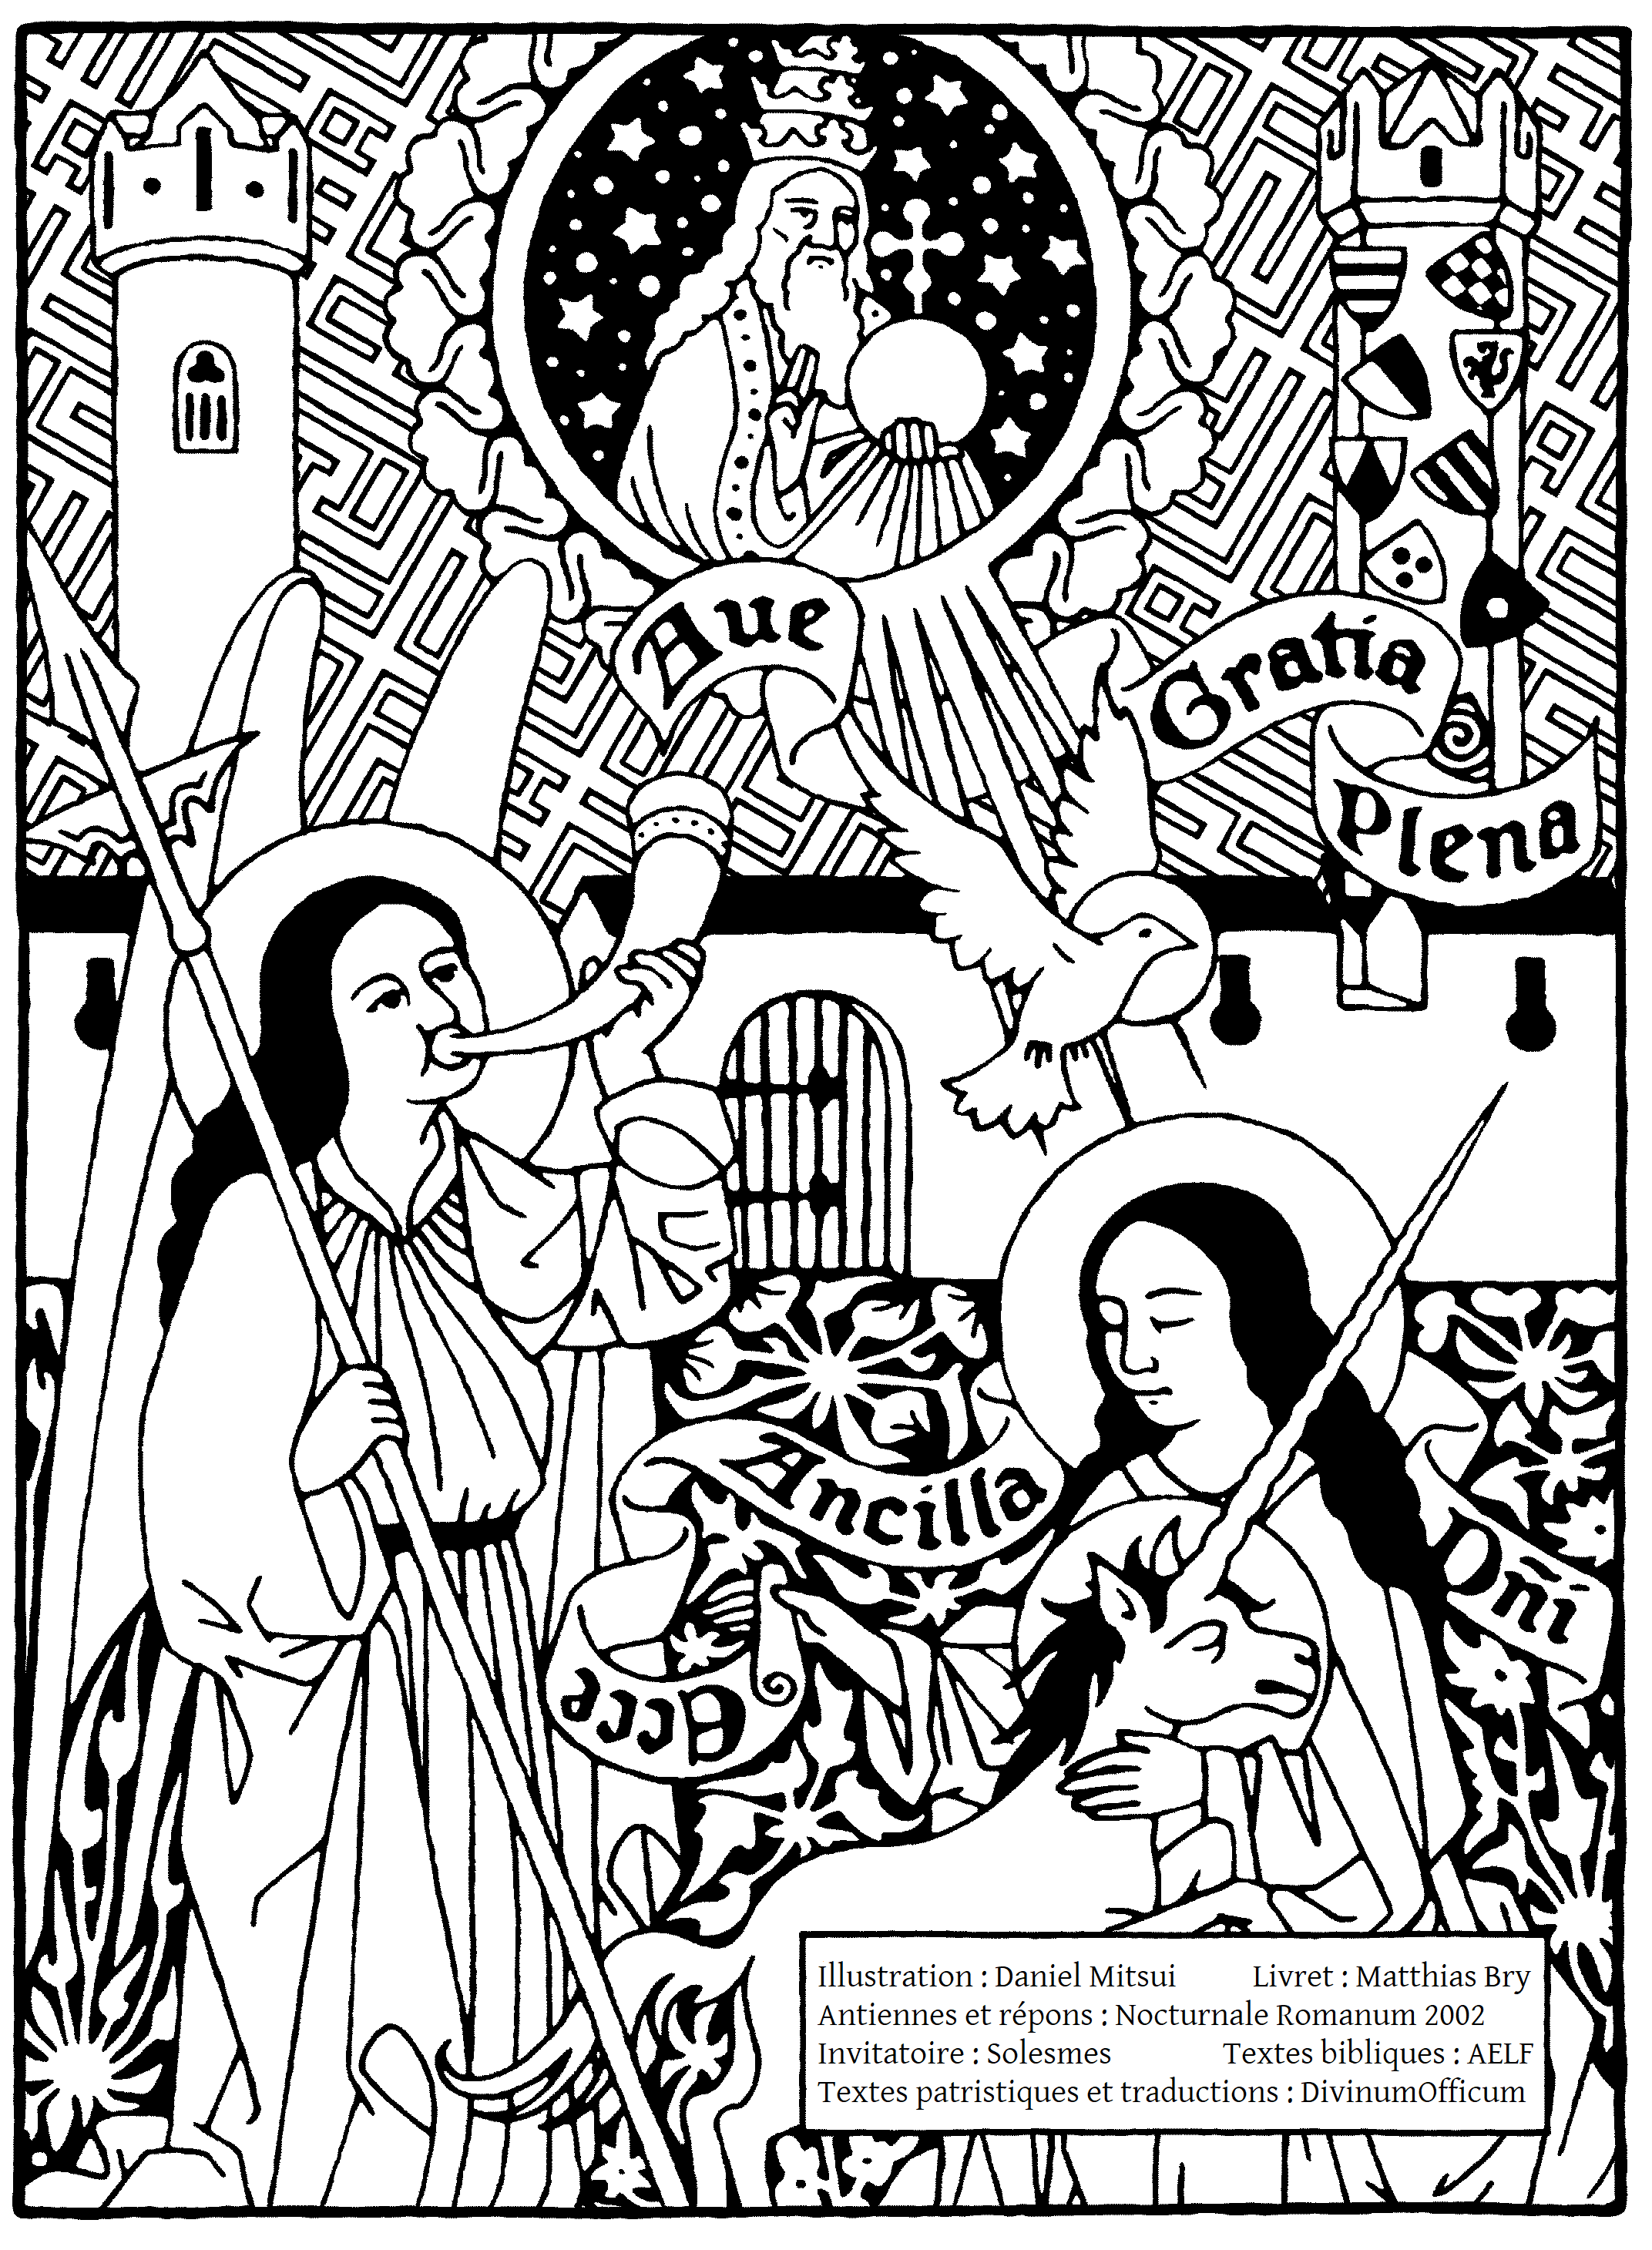
\includegraphics[width=13cm]{4ecouv.png}
\end{adjustwidth}
\end{document} 
